\documentclass[12pt,a4paper]{article}
\renewcommand{\baselinestretch}{1.5} 
\usepackage[utf8]{inputenc}
\usepackage{amsmath}
\usepackage{amsfonts}
\usepackage{amssymb}
\usepackage{titlesec}
\usepackage[edges]{forest}
\usepackage[parfill]{parskip}
\usepackage{listings}
\usepackage{natbib}
\usepackage{url}

\usepackage{geometry}
\geometry{a4paper, left=25.4mm, right=25.4mm, top=31.7mm, bottom=31.7mm}

\usepackage{graphicx}
\graphicspath{ {screenshots/} }

\setcounter{secnumdepth}{4}

\usepackage{color}

\definecolor{codegreen}{rgb}{0,0.6,0}
\definecolor{codegray}{rgb}{0.5,0.5,0.5}
\definecolor{codepurple}{rgb}{0.58,0,0.82}
\definecolor{backcolour}{rgb}{0.95,0.95,0.92}
\lstdefinestyle{sqlStyle}{
    backgroundcolor=\color{backcolour},
    commentstyle=\color{codegreen},
    keywordstyle=\color{magenta},
    numberstyle=\tiny\color{codegray},
    stringstyle=\color{codepurple},
    basicstyle=\footnotesize,
    breakatwhitespace=false,
    breaklines=true,
    captionpos=b, 
    keepspaces=true,
    showspaces=false,                
    showstringspaces=false,
    showtabs=false,
    tabsize=4,
    showlines=true
}

\def\hiddenparcommand{\par}
\newcommand\otherhiddenparcommand{\par\noindent}
\newcommand\hiddencommacommand{, }
\forestset{%
  declare keylist register={split here ids},% the list of nodes to split the tree at
  split here ids={},
  declare keylist register={split here interjects},% the list of comments to put in between the tree parts
  split here interjects={},
  declare keylist={split here auto siblings}{},% a list to hold the siblings which need edge restoration
  declare toks register=split here toks,
  declare dimen register=tmpdima,
  tmpdima'=0pt,
  declare dimen register=tmpdimb,
  tmpdimb'=0pt,
  declare dimen register=tmpdimc,
  tmpdimc'=0pt,
  to widest/.style={
    tikz+={\path (\forestregister{tempdima}, \forestoption{y}) -- (\forestregister{tempdimb}, \forestoption{y});},
  },
  hide commas/.style={%
    split here toks+={\hiddencommacommand},
    split here toks+={#1},
  },
  split dir tree pre/.style={%
    label={[text=gray, anchor=north, font=\scriptsize]below:{[cont.]}{}},
  },
  split dir tree post/.style={%
    label={[font=\scriptsize, anchor=south, text=gray]above:{[cont.]}{}},
  },
  split dir tree auto post/.style={% this gets applied to the first node after a break
    split dir tree post,
    tempkeylistc'={},
    tmpdimb/.option=y,
    for nodewalk={
      while={
        > ORw2+d _+d < On=! & {y}{tmpdimb}{##2-##1} {\textheight-#1} {n'}{1}%
      }{
        next,
        tempkeylistc/.option=name
      }%
    }{},
    % save the list
    split here auto siblings/.register=tempkeylistc,
    tikz+/.process={% this tries to redraw the edges to the following siblings
      OOw2{edge}{id}%
      {%
        \path [##1] (!u.parent anchor |- .north) ++(\forestregister{folder indent},1ex) coordinate (before ##2) |- (.child anchor);
        \edef\tempa{\foresteoption{split here auto siblings}}
        \foreach \i in \tempa \path [##1] (before ##2) |- ({forest cs:\i.child anchor});
      }%
    },
  },
  split dir tree/.code={%
    \forestset{%
      draw tree stage/.style={
        for root'={
          tempdima/.min={%
            >OOw2+d{x}{min x}{####1+####2}%
          }{tree},
          tempdimb/.max={%
            >OOw2+d{x}{max x}{####1+####2}%
          }{tree},
          for tree={%
            to widest,
          },
        },
        tempcountb'=-1,
        do until={%
          strequal((split_here_ids),"")
        }{%
          tempkeylistb'={},
          tempkeylista'={},
          split register={split here ids}{,}{tempcounta,tempkeylistb+},
          split register={split here interjects}{,}{temptoksa,tempkeylista+},
          split here ids'/.register=tempkeylistb,
          split here interjects'/.register=tempkeylista,
        % Sašo Živanović: http://chat.stackexchange.com/transcript/message/28484520#28484520
         for nodewalk={%
           draw tree processing order/.style={%
             filter={tree}{> ORw+n< OR> & {id}{tempcounta}{########1+1}{id}{tempcountb}}%
           }%
         }{},
          for root'={draw tree},
          TeX/.process={Rw{temptoksa}{\otherhiddenparcommand ####1\hiddenparcommand}},
          tempcountb'/.register=tempcounta,
        },
        for nodewalk={%
          draw tree processing order/.style={%
            filter={tree}{>OR>{id}{tempcountb}}%
          }%
        }{},
        for root'={draw tree},
      },
    }%
  },
  split dir here auto/.style n args=2{%
    split dir tree pre,
    !next node.split dir tree auto post=#2,
    split here ids+/.option=id,
%     !next node.split resume here ids+/.option=id,
    split={#1}{,}{split here toks,hide commas},
    split here interjects/.register=split here toks,
  },
  split dir tree auto/.style={%
    split dir tree,
    before drawing tree={%
      tempdima/.max={y}{tree},
      tempdimc/.register=tempdima,
      tempdimd/.min={y}{tree},
      tempdima-/.register=tempdimd,
      tempdimb'=\textheight,
      tmpdima'=10ex,
      tmpdimc'=\pagetotal,
      while={%
        >RR>{tempdima}{tempdimb}%
      }{%
        for nodewalk={%
          root',
          until={%
            > ROw2+d RRw2+d > {tempdimc}{y}{##1-##2} {tmpdima}{tmpdimc}{\textheight-##2-##1}%
          }{next node},
          previous node,
          split dir here auto/.process={R_w2{tmpdima}{}{{##2}{##1}}},
          next node,
          tempdima/.option=y,
          tempdimc/.register=tempdima,
          tempdima-/.register=tempdimd,
          tmpdima'=15ex,
          tmpdimc'=0pt
        }{},
      },
    },
  },
}


\begin{document}
	\begin{titlepage}
		\begin{center}
		
			B.Comp. Dissertation
			
			\vspace*{3.5cm}
			
			\fontsize{14pt}{14pt}\textbf {
			    Design and Implementation of a Location Based\\
                Data Tracking and Visualization Tool\\
                for Hardcore Traveller on iOS Platform\\
			}
			
			\vspace{4.5cm}
			
			By
			
			\vspace{0.5cm}
			
			Wang Jinghan
			
			
			\vfill
			
% 			Supervised by Prof. Wong Lim Soon
			
% 			\vspace{1cm}
			
			Department of Computer Science\\
			School of Computing\\
			National University of Singapore\\
			2016/2017
			
		\end{center}
	\end{titlepage}
	
	
	\pagenumbering{roman}
    \section*{Abstract}
    \addcontentsline{toc}{section}{Abstract}
    \clearpage
    
    
    \section*{Acknowledgment}
    \addcontentsline{toc}{section}{Acknowledgement}
    \clearpage
    
    
    \addcontentsline{toc}{section}{List of Figures}
    \renewcommand{\listfigurename}{List of Figures}
    \listoffigures
    \clearpage
	
	
	\tableofcontents


	\newpage


    \pagenumbering{arabic}
	\section{Introduction} % Lei
	    \subsection{Background}
	        \textit{``Well begun is half done''}, the ancient Greek philosopher Aristotle once wrote this in his work \textit{Politics}. Seventeen centuries passed, this famous proverb still applies in every single bits of people's life. As for travellers, the \textit{well begun} often comes from the thorough planning of their journey.
	        
	        One of the most effective way to plan the journey is by reading others' journals. Nowadays, travellers can easily find a huge amount of such kind of information on the traveling websites. Usually there are three categories of journals:
	        \begin{itemize}
                \setlength\itemsep{-0.5em}
                \item the ones with lots of photos and sights recommendations
                \item the ones with lots of personal thoughts and the understanding of different culture
                \item the ones with detailed plan and routes
            \end{itemize}
            
            We travelled a lot during the exchange period in Europe in 2016, the personal pain point from us is that when we are planning the journey, we can find tons of information of the first category listed above, but what we really need most is actually the third category. After the travellers have some places in mind, the problem they need to solve is to organize them properly so that they have sufficient time spent in each of the places and do not need to waste too much time traveling back and forth in between.
            
            There are various reason why we can rarely find information of the third category, one possible cause might be the difficulties of keeping track of everything regarding the routes and plans: as a traveller, one may clearly remember the different sights he visited, but seldom can he tell what time he left the hotel on the second day and how long did he spend on the bus from the hotel to the restaurant that he had lunch.
            
            To facilitate the traveller to keep the information of their detailed travel schedule, we come up with the idea of building the application using mobile phones with Global Positioning System (GPS) hardware to record and visualize the users' geo-location change within a period of time.
	  
	   \subsection{Overview}
	        Named after the Icelandic explorer Leifr Eiríksson, \textit{Leifr} is an iOS application to address the problem mentioned in the \textit{Background} subsection. The core functionalities of this application includes:
	        \begin{itemize}
                \setlength\itemsep{-0.5em}
                \item recording a path of user's geo-location information (longitude, latitude and altitude) with the exact time that this information is recorded
                \item visualize the visited places on the map and color it in a ``heat map'' manner to indicate how frequent the user visit a specify location
                \item view/share/replay a recorded path
            \end{itemize}
            
            There are also some advanced features implemented:
            \begin{itemize}
                \setlength\itemsep{-0.5em}
                \item replay all the paths sequentially starting from a selected date
                \item predict the location where the chosen photo is taken
                \item display the statistics about all the countries the user visited
            \end{itemize}
            
            Some of the extra features are planned to be implemented in the future, this will be discussed in the 5.3 \textit{Future Plans} subsection.
	        
	   \subsection{Comparison to Existing Products}
	        
    \clearpage
    
    
    \section{Use Cases and Demonstration}
        \subsection{View Aggregated Records} % Lei 
        % \includegraphics[width=0.3\textwidth]{test}
        \subsection{Record a New Path} % Lei
        \subsection{View All Recorded Paths} % Wang
            \subsubsection{Share a Recorded Path}
            \subsubsection{Paths Sharing}
        \subsection{Replay Paths} % Lei
            \subsubsection{Select Paths}
                \paragraph{Select a Path From Path Lists}
                \paragraph{Select Paths Starting From Some Date}
            \subsubsection{Playback Control}
        \subsection{Locate a Photo} % Wang
        \subsection{Check Statistics of Visited Countries} % Wang
    \clearpage    
    
    
    \section{Application Architecture} % 一起画
        % Class diagram and explanation
    \clearpage
    
    % Available technology discussion
    % Design choices
    % 
    \section{Development Details}
    
    As the title suggested, design and development are the two critical components of this project. In the previous section \textit{Application Architecture}, the high level structure of this application has been discussed. In this section, we will go into the details to discuss about the specific design decisions and the final implementation approaches for each individual feature. The whole section is categorized into front-end and back-end two parts, and the features of each part are listed accordingly. 
    
    \footnotesize
    This section is written jointly by Jinghan and Mingyu. Please refer to the individual subsections for specific attributions.
    \normalsize
            
        \subsection{Front-End Details}
        There are seven general features in terms of front end development. The first subsection \textit{Fundamentals} will discuss the overall view hierarchy while the rest will keep the focus on different views.
            
            \subsubsection{Fundamentals} % Wang
            \label{fe:fundamentals}
            Based on the well accepted model-view-controller pattern, Apple has provided several standard templates for developers to organize the views in their applications. In general, developers are recommended to use these template to take advantages of the built-in optimisation. Among the various template provided, we picked out the ones we may potentially make use of:
            \begin{itemize}
            \setlength\itemsep{-0.5em}
            \item master-detail application template
            \item page-based application template
            \item tabbed application template
            \end{itemize}
            
            The master-detail application template provides a convenient starting points for data driven applications where only brief data are shown in a list. Users will only view the details when they click on a specific list item. \texttt{UITableView} as the list view (master), is the perfect fit when showing texts or simple images, but when the geo-location data come in, the list introduces too much cognitive load to the viewer. 
            
            In the page-based and tabbed application template, there are no cognitive hassles as in master-detail template when displaying geo-location data. However, in neither of these two, there is no native accommodations for the controls. A naive solution maybe in each essential view (i.e. each page in a page-based template or each tab in a tabbed template), we put the relevant controls directly on top. This will certain solve the problem, but at the cost of messing up the user's working space. Furthermore, there are possibly cases where one single control needed to be shared among different pages or tabs, but with this naive solution we will have to duplicate the codes here and there.
            
            Due to the fact that none of the templates suit our needs, we decided to implement our own view hierarchy. The customized scheme we proposed (and implemented) can be considered as an extension of the tabbed application template. The main difference is that in our hierarchy, the tab bar can be pulled up and reveal the control panel, where various controls are placed. The controller of each essential view will inherit from a common parent view controller, which implements a protocol to delegate the data sources of the controls. When a control needs to be shared among different views, it is defined in the parent view controller. When a control is only needed in one single particular view, it is defined in the specific child view controller. In this way, we avoid the potential duplicated codes. Furthermore, the customized tab bar is able to snap into several code-defined levels so that a control may only be shown when it is really needed by the user. Figure \ref{fig:fundamental} shows the customized tab bar in different snapping levels.
            
            \footnotesize
            Section \ref{fe:fundamentals} is written by Jinghan.
            \normalsize
            
            \begin{figure}
                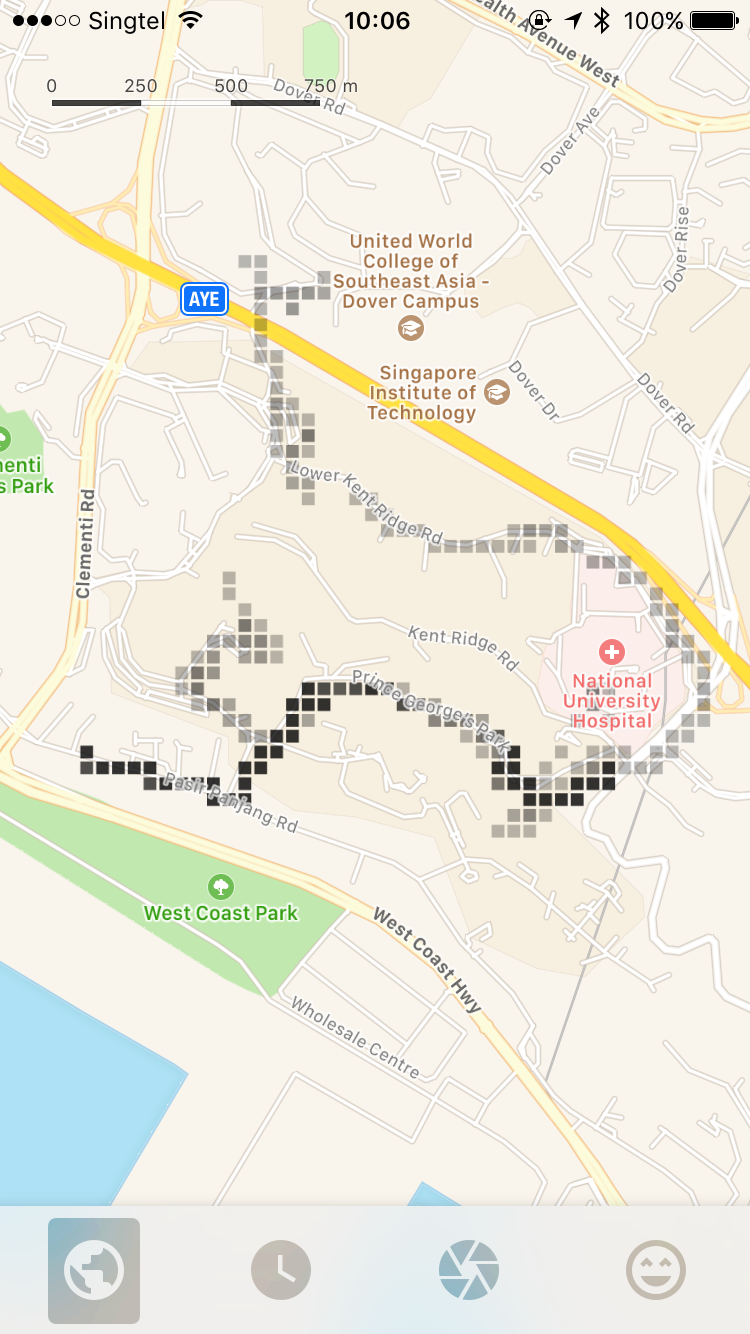
\includegraphics[width=0.32\textwidth]{4-1-1-a}
                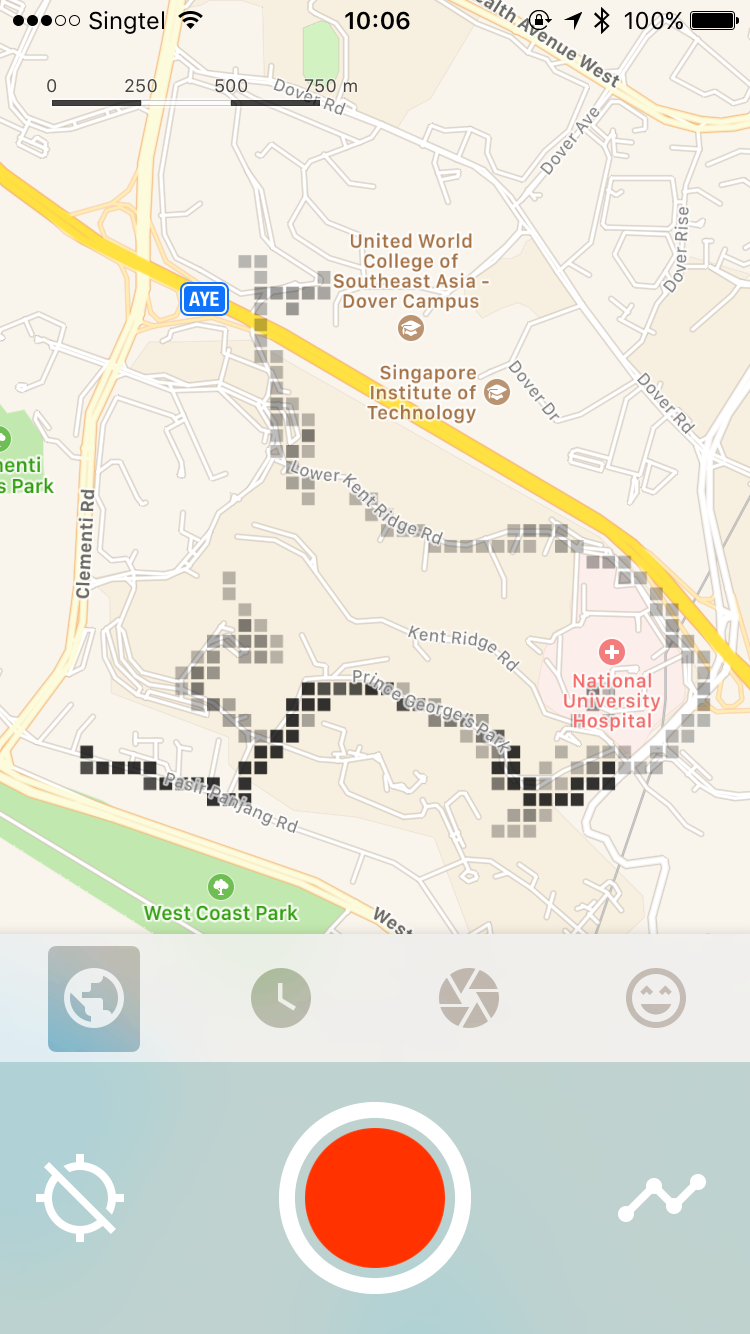
\includegraphics[width=0.32\textwidth]{4-1-1-b}
                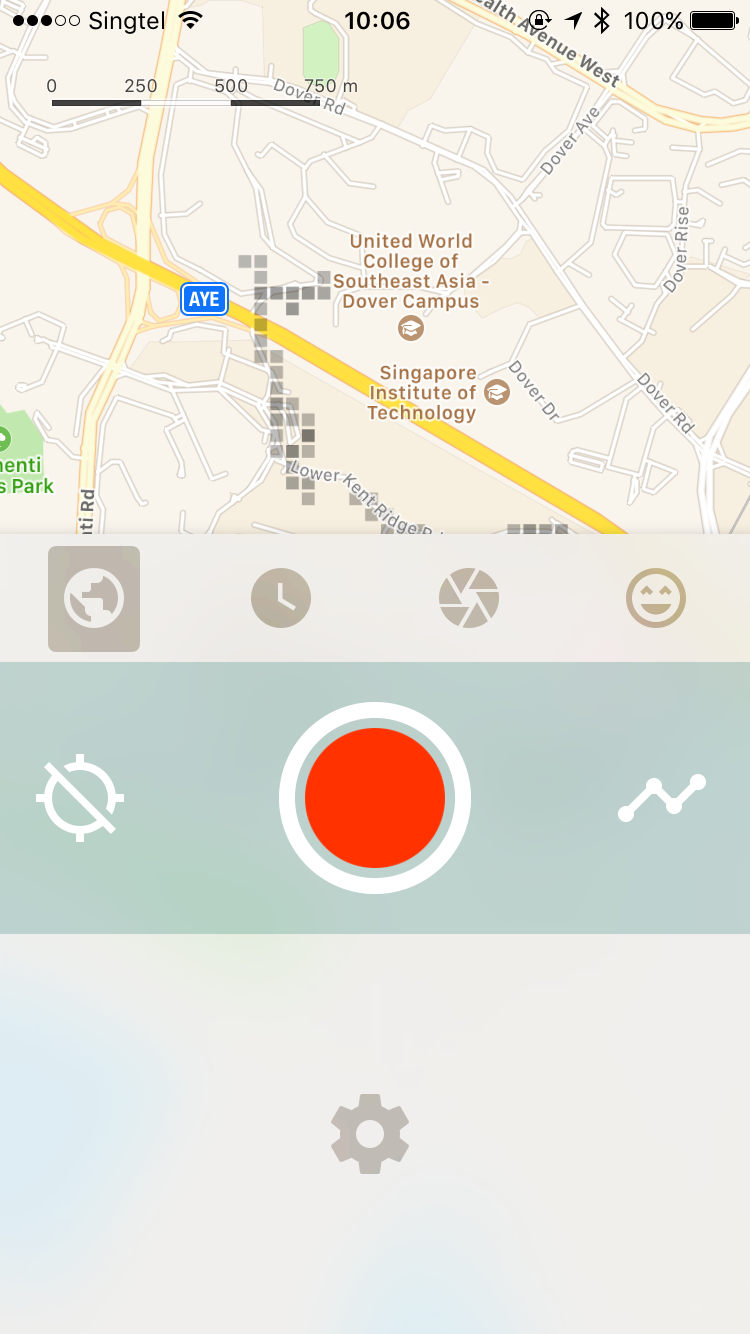
\includegraphics[width=0.32\textwidth]{4-1-1-c}
                \centering
                \caption{Customized tab bar at different snapping levels}
                \label{fig:fundamental}
            \end{figure}
            
            \subsubsection{Geo-Location Information Recording} %
            \label{fe:geolocation-information-recording}
            The core features of this application are based on the data collected from the path recording. In the application, a singleton manager \texttt{LFGeoRecordManager} is dedicated to all the services involving geo-location recording. When the user switch on the recording, the flag \texttt{isRecording} in \texttt{LFGeoRecordManager} will be set to \texttt{true}, this flag is checked in the several places like the history view controller for current path overlay drawing (see 4.1.3 \textit{History Overview}) and in the \texttt{AppDelegate} when the \texttt{CLLocationManager} detects an update of the current location: if the flag is on, the \texttt{LFGeoRecordManager} encapsulates the coordinate of the new location and the time information into a abstracted model \texttt{LFPoint} and append it to a buffer path. The reason behind this buffer path idea is that the database access time is significantly longer than manipulating a memory-level variable, by buffering the incoming new geo-location information and flushing the path into database regularly, frequent database access is avoided. The interval between each flushing is 600 seconds and the user can also perform manual flushing in the settings page (see \ref{fe:settings} \textit{Settings}). Once the recording is stopped by the user, the current buffer path will be flush as well.
            
            In the \texttt{LFGeoRecordManager}, a mutex is applied to ensure that appending a point and flushing the existing points won't happen simultaneously.
            
            \footnotesize
            Section \ref{fe:geolocation-information-recording} is written by Mingyu.
            \normalsize
            
            \subsubsection{History Overview}
                \paragraph{Map Framework} % Lei/mapbox dynamic updates
                \paragraph{Rendering Details} % Wang
            \subsubsection{Path Lists} % Lei
            \subsubsection{Path Playback} % Lei 
            \subsubsection{Photos} % Wang
            \subsubsection{Statistics} % Wang
            
            \subsubsection{Settings} % Lei
            \label{fe:settings}
            In subsection \ref{fe:fundamentals} \textit{Fundamentals}, it's mentioned that the customized tab bar has different snapping levels, the first level of tab item is the specific control panel for each of the views, and the second one is the homogeneous settings entry point. Currently only two features are implemented in the settings page:
            \begin{itemize}
                \setlength\itemsep{-0.5em}
                \item Reconstruct database
                \item Flush buffer path
            \end{itemize}
            \paragraph{Reconstruct Database}
            Occasionally, some corrupted data might be introduced in the cached database, since the rendering of path history view is based on the data stored in the cached database, corrupted cached data could cause incorrect rendering result. Therefore, the user is provided a way to recover the cached data from the main SpatiaLite database.
        
            Since the reconstruction process is iterated zoom level by zoom level, it is not efficient to make the reconstruction back-end method to interact with the front-end progress view after every single point is migrated; the progress view should be updated level by level as well. There are two possible simple progress percentage calculation algorithm can be adopted here:
            \begin{itemize}
                \setlength\itemsep{-0.5em}
                \item Calculate the percentage from the completed levels and total levels (21 in this application map settings):
                \begin{equation}
                    p = \frac{n_c}{21}\times100\%
                \end{equation}
                where $p$ is the progress percentage and $n_c$ is the completed levels.
                \item Calculate the percentage from the estimated completed points and the total completed points; since the rendered grid size is calculated by:
                \begin{equation}
                    s = \frac{1}{2^{n}}\cdot\frac{w}{10240000}
                \end{equation}
                where $s$ is the grid size, $n$ is the zoom level and $w$ is the width for MapKit world size.
                
                It can be assumed that estimated number of points in level $n$ will have four times of points in level $n+1$.
                
                Thus the estimated progress percentage can be calculated as:
                \begin{equation}
                    p = \frac{4^{n_c}}{4^{21}}\times100\%
                \end{equation}
                where $p$ is the progress percentage and $n_c$ is the completed levels.
            \end{itemize}
            
            Since fewer points are associated with smaller zoom level, if the progress percentage is calculated following the first algorithm above, the progress view will go much faster at the beginning, then slow down as the reconstructing zoom level becomes larger. This gives the user a false hope that the reconstruction will finish shortly but the outcome is that it goes slower and slower. It is not a good user experience and the feedback information from the progress view is not accurate. The problem can be addressed with the second algorithm; although the number of points is still under estimation, it is more accurate since the different numbers of points in each zoom level are taken into consideration.
            
            For more information regarding the cached database and database reconstruction, see relevant section \ref{db:fundamentals} \textit{Fundamentals} and \ref{db:realm} \textit{Realm}.
            
            \paragraph{Flush Buffer Path}
            This is where the user can be manual buffer path flushing discussed in section \ref{fe:geolocation-information-recording} \textit{Geo-Location Information Recording}.
            
            \footnotesize
            Section \ref{fe:settings} is written by Mingyu.
            \normalsize
            
            
            \begin{figure}
                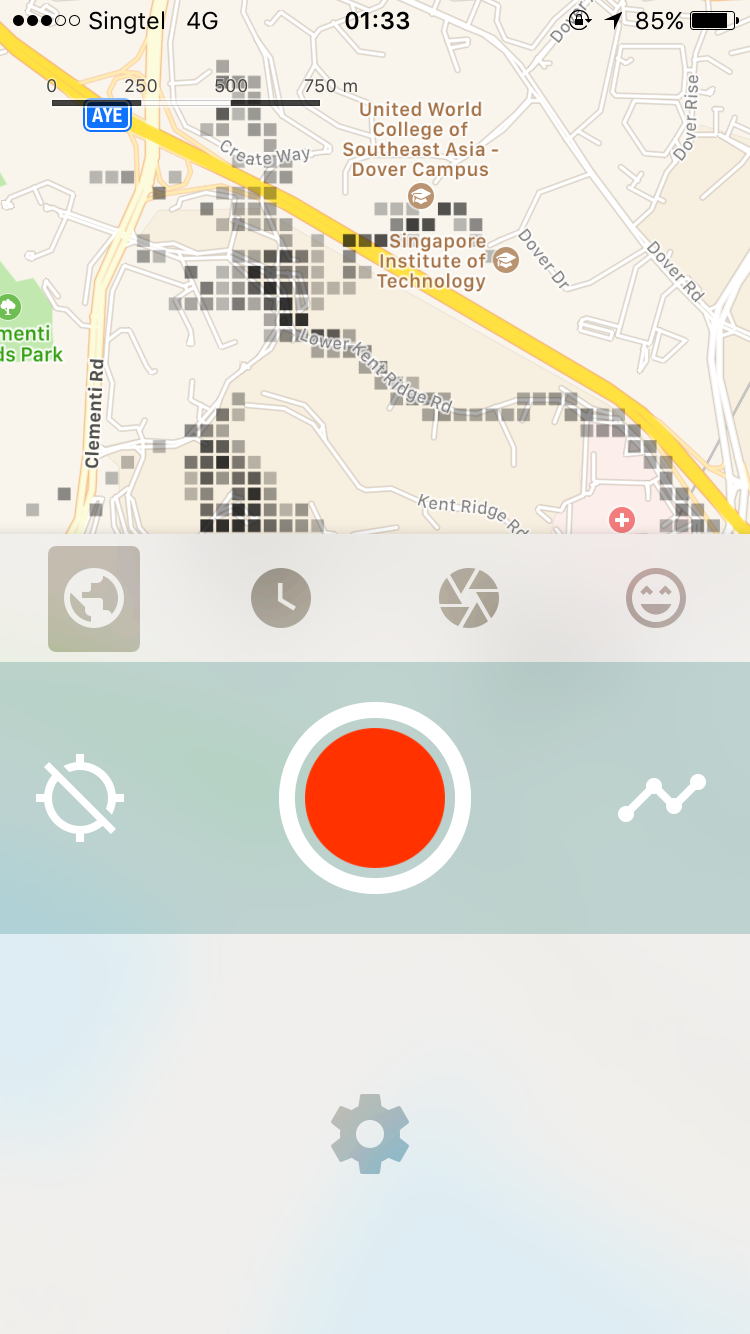
\includegraphics[width=0.32\textwidth]{4-1-8-a}
                
\includegraphics[width=0.32\textwidth]{4-1-8-b}
                
\includegraphics[width=0.32\textwidth]{4-1-8-c}
                \centering
                \caption{Settings page and reconstruct database}
                \label{fig:settings}
            \end{figure}
            
        \subsection{Back-End Details}
        There are five subsections regarding the back-end development details. The first subsection \textit{Fundamentals} will critique the available options and discuss how we ended up with our current back-end architecture. The rest will concentrate on the discussion of how we apply different technologies to implement the design.
        
            \subsubsection{Fundamentals} % Wang
            \label{db:fundamentals}
            Before we diving into the discussion on our choices among the available database technologies and the rational behind those choices, a restatement of the requirements would be helpful for making clear of what are the desired features. The following are the features that require data persistence support and their corresponding requirements for the data persistence module:
            \begin{itemize}
            \setlength\itemsep{0em}
            \item showing the aggregated path records:
                \begin{itemize}
                    \setlength\itemsep{-0.5em}
                    \item requires massive aggregation operations through the entire database
                    \item requires querying according to geological regions (longitude and latitude)
                    \item requires outputs to be bounded (otherwise front end may be overwhelmed)
                    \item compromise on precision may be acceptable depending on zoom scales
                \end{itemize}
            \item showing path records according to time
                \begin{itemize}
                    \setlength\itemsep{-0.5em}
                    \item requires querying according to time
                    \item requires loss-less precision on a selected portion of the data
                \end{itemize}
            \item showing local photos
                \begin{itemize}
                    \setlength\itemsep{-0.5em}
                    \item requires querying according to time (locations)
                    \item requires fast loading of massive data (photos)
                    \item requires querying on different resolutions (photos)
                \end{itemize}
            \item importing and exporting for path sharing
                \begin{itemize}
                    \setlength\itemsep{-0.5em}
                    \item requires convenient access to portable files
                    \item requires secure serialization
                    \item requires easy separation between shared paths and regular paths
                \end{itemize}
            \end{itemize}
            
            According to the requirements specified above, the application overall requires 3 different data persistent components: 
                \begin{enumerate}
                    \setlength\itemsep{-0.5em}
                    \item a component as the essential component to persist users' regular records
                    \item a component to manage the photos
                    \item a component to manage the incoming and outgoing path files
                \end{enumerate}
            Apple has provided some well-established, native solutions for Component 2 and 3 and they can fit into our case very well. Therefore, the design choices are clear regarding these two and we will discuss them in detail in subsection \ref{db:photo} and \ref{db:direct-files}. However, for Component 1, there is no clear solution to address all the requirements listed. Some of available technologies we have researched include Core Data, SQLite, Realm and SpatiaLite.
                
            Core Data is one of the most popular data persistent approach on iOS. It is provided and maintained by Apple and integrated into the operating system natively. The large user base of Core Data results in a very comprehensive community to seek help from. However, Core Data is not designed as a database, but an object graph manager. Therefore, a lot of functions in Core Data are aiming to make the object relationships accessible and organized rather than pursuing high performances. In our case, the only entities are point, path and country, a complicated object graph manager is therefore not required.
            
            SQLite is the base of Core Data, but without all the object graph management overhead. So naturally, if Core Data was not suitable enough, the lower level SQLite turns to be the second consideration. SQLite is also supported natively by iOS and it is faster than Core Data, but as we taking out the Core Data wrapper, raw SQLite is much harder to setup and use. There will have to be vast number of manipulations on C pointers in Swift, which are often tedious, unintuitive and messy. Moreover, SQLite by default does not support multi-threading. In our use case, when the map is loading, each tile will load from a different thread. If the database module can only be accessed from a single thread, all database requests would then have to be lined up in a queue, which defeats the original purpose of the map's multi-thread loading. Furthermore, with SQLite, we would have to write the SQL statements in the form of strings, which is error-prone and sometimes maybe hard to debug. All these hassles made us wonder whether there’s a better choice.

            Realm is the next one we examined. This is a much younger framework comparing to SQLite. In general, there are three characteristics of Realm to make it particularly attractive to us. Firstly, Realm operates in a synchronous, but lazy manner. This is important to us because when loading the map tiles, the life time of each loading thread is controlled by the OS rather than ourselves. Asynchronous loading may result in a condition that the thread is deallocated before the data arrives. Secondly, in Realm, data are exposed as objects and thus it can fit into our objective oriented codes very easily. This appears even more appealing when comparing to the complicated setup and querying steps of SQLite. Thirdly and most importantly, Realm is fast. Figure \ref{fig:database-performance} shows the performance comparison between Realm and other popular data persistence solutions including SQLite and Core Data. \citet{DatabasePerformanceFigure}
            
            
            \begin{figure}
                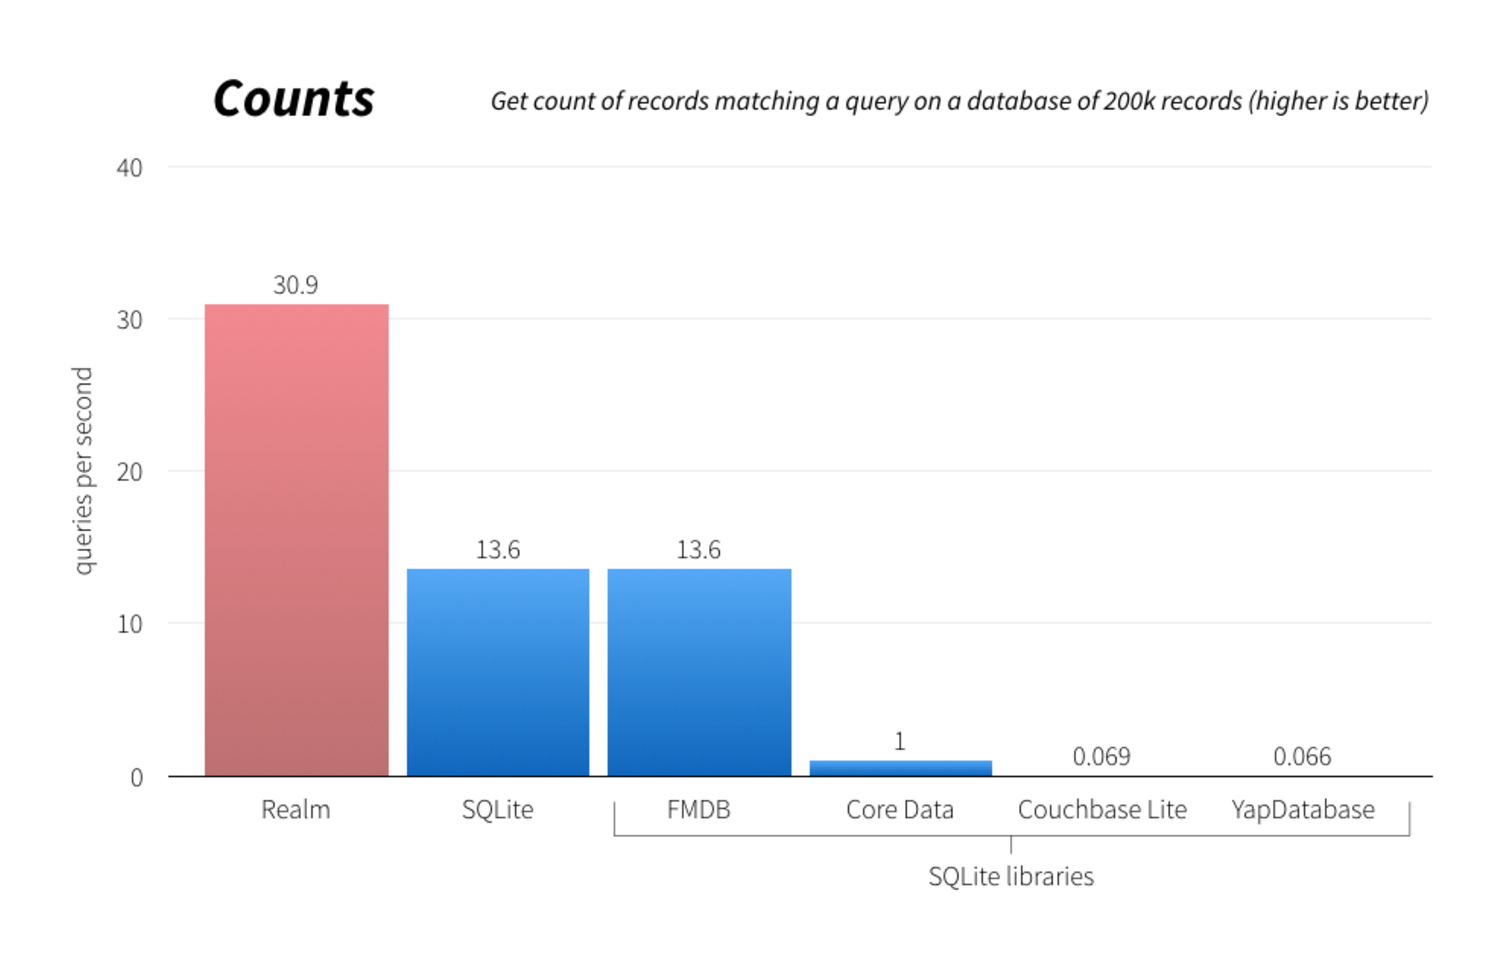
\includegraphics[width=0.49\textwidth]{4-2-1-a}
                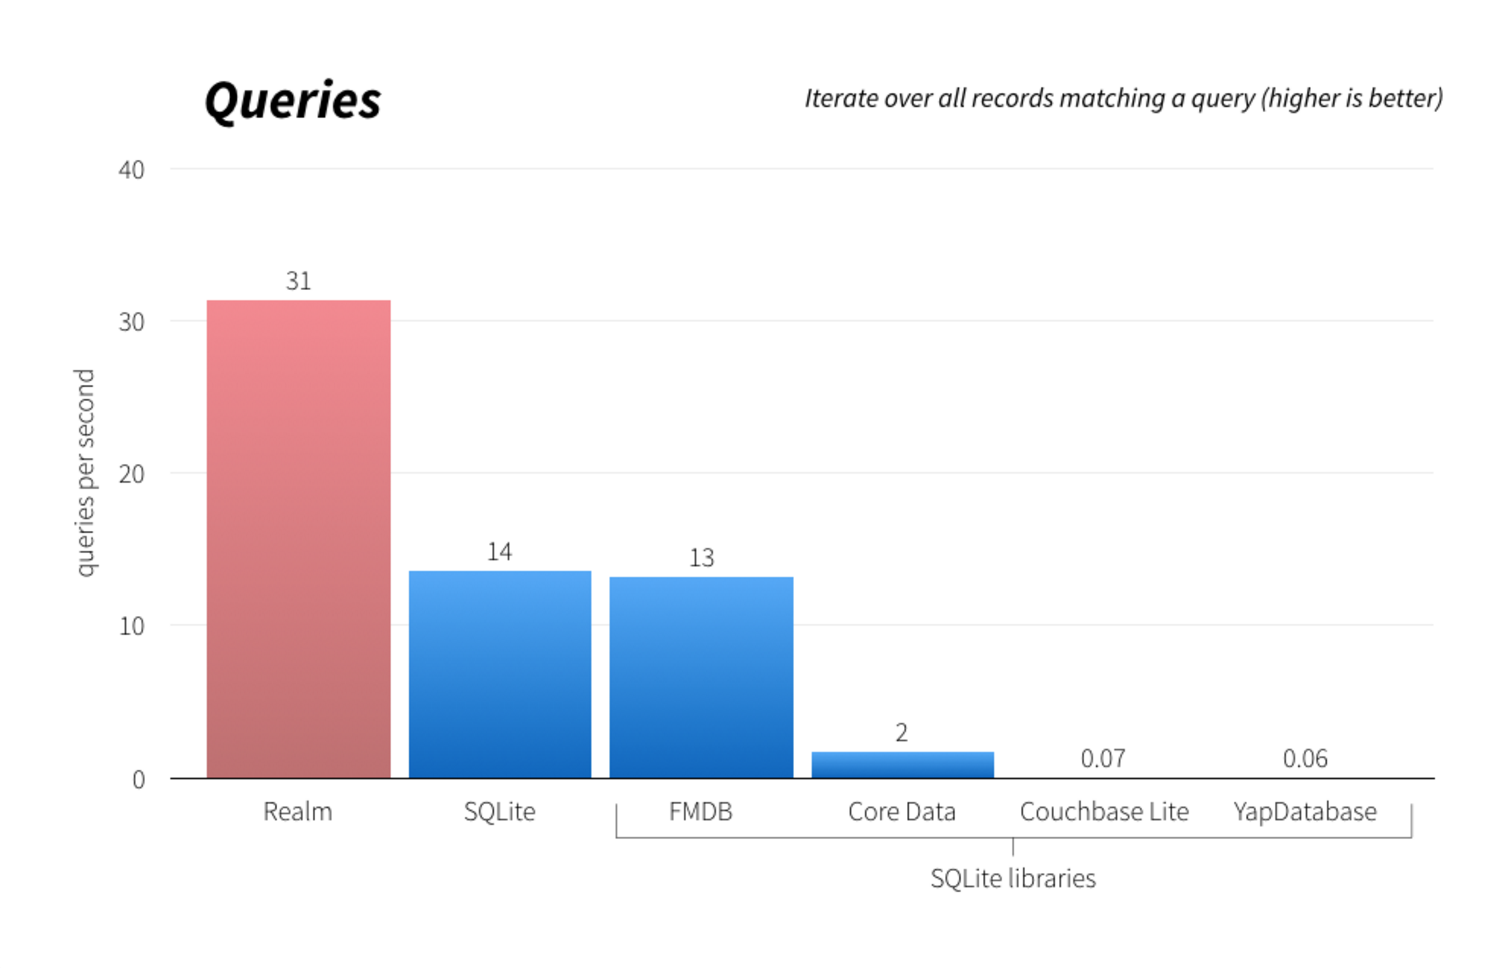
\includegraphics[width=0.49\textwidth]{4-2-1-b}
                \centering
                \caption{Performance comparison between Realm and other solutions}
                \label{fig:database-performance}
            \end{figure}
            
            Realm manages to address most of our requirements, however, there is still no way to perform appropriate samplings. As mentioned in the requirement, we would like the database omits some of the records based on the zoom scale on which the query is performed. With the consideration of this should be a common requirement for every application that deals with massive geo-location data, we started searching for specialized spatial databases to fulfill our needs.
            
            SpatiaLite is the only spatial database we found which can be integrated into an iOS application without too much hassles. It supports all the required spatial functions, such as simplifying paths and snapping points to grid, in order to perform the sampling task. However, as an extension of SQLite, SpatiaLite suffers from the same sets of problems as SQLite, and most of the time, the problems tend to be more severe due to its small user base and poor documentation.
            
            There is no single perfect solution here to fully address all requirements at once, but fortunately, we don't have to stick with only one of these options. A combinatorial scheme is to use SpatiaLite as the base-level database for storing and processing every detail of the recorded user data, and then to use Realm as a cache database in between to allow fast querying on the processed data when loading up the map. When new data entries arrives, it will be first stored into the base database, then the base database perform the aggregation operations and update the cache database with the new result. In this way, computations are kept decentralized and thus the querying performance is improved. In the extreme cases where some inconsistencies occur between the two databases, it is also possible to reconstruct the entire cache database from scratch. The combinatorial scheme finally fulfilled all the requirements, and thus, it is chosen as our final solution on the data persistence component design.
            
            \footnotesize
            This section is written by Jinghan.
            \normalsize
            
            \subsubsection{SpatiaLite} % Wang
            As mentioned in section \ref{db:fundamentals}, SpatiaLite is used as the base database that stores and processes all recorded geo-location and time data. The only table here is table \texttt{tracks}, the schema of which is shown in Figure \ref{fig:schema}.
            
            \begin{figure}
                \lstset{style=sqlStyle}
                \centering
                \lstinputlisting[language=SQL]{others/schema.sql}
                \caption{SQL schema for table \texttt{tracks}}
                \label{fig:schema}
            \end{figure}
                
                \paragraph{Spatial Attributes and Functions}
                SpaitiaLite allows eight geometry types in the table, namely, \texttt{GEOMETRY}, \texttt{POINT}, \texttt{LINESTRING}, \texttt{POLYGON}, \texttt{MULTIPOINT}, \texttt{MULTILINESTRING}, \texttt{MULTIPOLYGON} and \texttt{GEOMCOLLECTION}. Among the eight types, \texttt{POINT} and \texttt{LINESTRING} are considered as the most relevant ones. As you might have already noticed from Figure \ref{fig:schema}, we store the geo-location data as tracks. Each track is made up of a \texttt{LINESTRING} and an identifier. Each \texttt{LINESTRING} consists of one or more four-dimensional \texttt{POINT}s, and the four dimensions of every single \texttt{POINT} are: longitude, latitude, altitude and time.
                
                \paragraph{WKB, WBT and GeoJSON}
                
                
            \subsubsection{Realm} % Lei
            \label{db:realm}
            \subsubsection{Photos} % Wang
            \label{db:photo}
            \subsubsection{Direct Files} % Wang
            \label{db:direct-files}
    \clearpage
    
    
    \section{Conclusion} 
        \subsection{Summary} % Lei 
        \subsection{Difficulties and Limitations} % Wang
        % WKT WKB, spatialite init, spatialite document, remove screenshots
        \subsection{Future Plans} % Lei
        \subsection{Commercial Potentials} % Wang
    \clearpage
    
    
    \pagenumbering{roman}
    \setcounter{page}{10} % 记得改!!!!!
    
    \section*{Project Contribution}
    \addcontentsline{toc}{section}{Project Contributions}
    \clearpage
    
    
    \addcontentsline{toc}{section}{References}
    \bibliographystyle{apalike}
    \bibliography{others/refs}
    \clearpage
    
    
    \subsection*{Appendix A - Program Listing}
    \addcontentsline{toc}{section}{Appendix A - Program Listing}
    \begin{forest}
        for tree={
            folder,
            grow'=0,
            fit=band,
            font=\ttfamily,
        },
        split dir tree auto,
        [LEIFR
            [Views
                [Cells
                    [LaunchScreen.storyboard]
                    [Main.storyboard]
                    [LFHistoryControlView.xib]
                    [LFPlaybackControlView.xib]
                    [LFPlaybackCalendarView.xib]
                    [LFPhotoControlView.xib]
                    [LFRecordButton.swift]
                    [LFNavigationBar.swift]
                    [LFPlayBackAnnotationView.swift]
                    [LFSettingAccessoryView.xib]
                    [Table View Cells
                        [LFTableViewCell.swift]
                        [LFTableViewCell.xib]
                        [LFButtonCell.swift]
                        [LFButtonCell.xib]
                        [LFImageCell.swift]
                        [LFImageCell.xib]
                        [LFMapCell.swift]
                        [LFMapCell.xib]
                        [LFTrackTableViewCell.swift]
                        [LFTrackTableViewCell.xib]
                        [LFInboxTableViewCell.swift]
                        [LFInboxTableViewCell.xib]
                    ]
                    [Collection View Cells
                        [LFCollectionViewCell.swift]
                        [LFCollectionViewCell.xib]
                        [LFCollectionViewCell.swift]
                        [LFCollectionViewCell.xib]
                        [LFGridViewCell.swift]
                        [LFGridViewCell.xib]
                        [LFHorizontalCollectionViewCell.swift]
                        [LFHorizontalCollectionViewCell.xib]
                        [LFFlagCollectionViewCell.swift]
                        [LFFlagCollectionViewCell.xib]
                        [LFStatisticsCollectionViewCell.swift]
                        [LFStatisticsCollectionViewCell.xib]
                    ]
                ]
            ]
            [Renderers
                [LFGeoPointsOverlayRenderer.swift]
                [LFCurrentPathOverlayRenderer.swift]
            ]
            [Extensions
                [UIKitExtension.swift]
                [LFConstant.swift]
                [MapKitExtension.swift]
            ]
            [Models
                [LFPath.swift]
                [LFPoint.swift]
                [LFCachedPoint.swift]
                [LFCachedLevel.swift]
                [LFCachedCountry.swift]
                [LFIncomingPath.swift]
            ]
            [Services
                [LFDatabaseManager.swift]
                [LFGeoRecordManager.swift]
                [LFGeoJSONManager.swift]
                [LFCachedDatabaseManager.swift]
                [LFPhotoManager.swift]
                [LFReverseGeocodingManager.swift]
                [LFLocalFileManager.swift]
                [LFPathsPlayingManager.swift]
                [LFPathPlayingManager.swift]
            ]
            [ViewControllers
                [Base
                    [LFLoadingViewController.swift]
                    [LFSettingViewController.swift]
                    [LFViewController.swift]
                    [LFHoverTabBaseController.swift]
                    [LFHoverTabViewController.swift]
                ]
                [Tab 1
                    [LFHistoryViewController.swift]
                    [LFTrackTabViewController.swift]
                    [LFMyTrackViewController.swift]
                    [LFInboxViewController.swift]
                ]
                [Tab 2
                    [LFPlaybackViewController.swift]
                    [LFPlaybackCalendarViewController.swift]
                ]
                [Tab 3
                    [LFPhotoViewController.swift]
                    [LFPhotoDetailViewController.swift]
                ]
                [Tab 4
                    [LFStatisticsViewController.swift]
                    [LFFlagViewController.swift]
                    [LFStatisticsCollectionViewController.swift]
                    [LFStatisticsViewLayout.swift]
                    [LFMapPreviewViewController.swift]
                ]
            ]
        ]
    \end{forest}
    \clearpage
    
    \subsection*{Appendix B - Installation Guide}
    \addcontentsline{toc}{section}{Appendix B - Installation Guide}%
    \clearpage
    

\end{document}